\chapter{第一个程序}
\label{ch:01}

万事开头难，但这一章只干三件事：把工具装好、跑出一行字、看懂这行字是怎么来的。

读完这一章，你会有第一个能跑的程序，也会知道「出错」在 Magel 里长什么样——后者比前者重要，因为接下来每一章你都会用到它。

\section{把工具装好}

Magel 只有一个命令行程序，叫 \texttt{magel}，解释、编译、建工程、跑测试全在它里面。装它有两条路。

这条路最短：用发布包。 拿到 \texttt{dist/\allowbreak{}magel-<\allowbreak{}版本>\allowbreak{}-<\allowbreak{}平台>\allowbreak{}-<\allowbreak{}架构>\allowbreak{}.\allowbreak{}tar.\allowbreak{}gz}，解开，把里面的 \texttt{bin/\allowbreak{}} 加进 PATH，就完事了。

这条路最全：从源码构建。 适合想改编译器的人，也适合想看清内部的人：

\par
\medskip
\begin{lstlisting}[style=sh]
sh gen.sh      # 用 IELR 从 magel.gram 生成前端
make           # 构建 magel 与 libparser.a
\end{lstlisting}
\par
\medskip

\texttt{gen.\allowbreak{}sh} 需要一份 \href{https://github.com/rabbitc999/ParseEngine}{ParseEngine} 文法生成器，细节见\href{https://gitee.com/rabbitc999/magel/blob/master/doc/01-quickstart.md#1-安装}{快速开始}，这里不展开。

装完了，敲一句：

\par
\medskip
\begin{lstlisting}[style=sh]
magel help
\end{lstlisting}
\par
\medskip

屏幕上滚出一大串用法，就说明装好了。先别急着读完那串帮助——那是给有经验的人查的，跟着这本书走，你会一个个认识里面的选项。

\begin{tip}{Windows 用户注意}
程序名是 \texttt{magel.\allowbreak{}exe}。在 Git Bash / MSYS 里写 \texttt{.\allowbreak{}/\allowbreak{}magel} 能自动找到 \texttt{magel.\allowbreak{}exe}；光写 \texttt{magel} 会去 PATH 里找，可能找到的不是你当前目录这一份。本书后文一律写 \texttt{magel}，你自己敲的时候按环境补上 \texttt{.\allowbreak{}/\allowbreak{}}。
\end{tip}

\section{Hello, Magel}

新建一个文件 \texttt{hello.\allowbreak{}mgl}，内容如下：

\par
\medskip
\begin{lstlisting}[style=magel]
int64 main()
{
    println("Hello, Magel!");
    return 0;
}
\end{lstlisting}
\par
\medskip

\par
\medskip
\begin{lstlisting}[style=out]
Hello, Magel!
\end{lstlisting}
\par
\medskip

然后运行它：

\par
\medskip
\begin{lstlisting}[style=sh]
magel run hello.mgl
\end{lstlisting}
\par
\medskip

屏幕上出现 \texttt{Hello,\allowbreak{} Magel!}，第一个程序就成了。

\texttt{magel run} 这个写法看着啰嗦，其实 \texttt{run} 是可以省的——直接

\par
\medskip
\begin{lstlisting}[style=sh]
magel hello.mgl
\end{lstlisting}
\par
\medskip

效果一样。但本书会一直写 \texttt{magel run}，因为把场景写出来在人多的时候少很多误会：\texttt{magel hello.\allowbreak{}mgl Alice} 和 \texttt{magel run hello.\allowbreak{}mgl Alice} 是同一件事，但 \texttt{magel check hello.\allowbreak{}mgl} 完全是另一件事。

\section{逐行看懂它}

就三行，一行一行来。

第一行：\texttt{int64 main(\allowbreak{})\allowbreak{} \{}

程序从哪里开始跑？从 \texttt{main} 开始。这个名字是定死的，不能改成 \texttt{Main}、\texttt{start} 或者别的什么。前面的 \texttt{int64} 是它返回的东西的类型，\texttt{(\allowbreak{})\allowbreak{}} 里现在空着，意思是它不接收参数。

\texttt{int64} 是一种整数类型：能装 64 位的有符号整数，大概正负九百多万亿。为什么入口要返回一个整数？因为操作系统想看它：返回 \texttt{0} 表示「正常结束」。你在终端里看到的 \texttt{echo \$?}，读的就是这个值。

第二行：\texttt{println(\allowbreak{}"Hello,\allowbreak{} Magel!")\allowbreak{};}

\texttt{println} 是「打印一行」的意思：把括号里的东西写到屏幕上，末尾自动换行。它是 Magel 核心库里最常用的函数，不用 \texttt{import} 就能用。

行尾那个 \texttt{;} 是分号，表示这句话说完了。跟 C、Java 一样。

第三行：\texttt{return 0;}

告诉操作系统「我正常结束了」，然后交还控制权。

最后的花括号 \texttt{\}} 是 \texttt{main} 的结尾。

看出来了吗——花括号划范围，分号断句，这和 C 系语言一模一样。这是 Magel 刻意这么做的：你已经会的东西，它不想让你重学一遍。

\section{\texttt{run} 和 \texttt{check}}

现在故意把程序弄坏一次，看看会发生什么。把第二行末尾的分号删掉：

\par
\medskip
\begin{lstlisting}[style=magel]
int64 main()
{
    int64 x = 1
    return 0;
}
\end{lstlisting}
\par
\medskip

再跑：

\par
\medskip
\begin{lstlisting}[style=out]
语法错误：hello.mgl 第 3 行第 5 列：期望 条件(if) / 自增(++) / 自减(--) / 加号(+) 等 44 个之一，实际是 返回(return)
 3 |     return 0;
   |     ~~~~~~
\end{lstlisting}
\par
\medskip

三件事值得注意：

\begin{itemize}

\item 它告诉你第 3 行第 5 列，还把出问题的那段源码抄给你、底下画上波浪线。第 1 行少了个分号，报的却是第 3 行——这是解析器在往后看：它读完第 2 行还在等一个分号，结果等来了 \texttt{return}，于是「在 \texttt{return} 这里」断了。看到报错位置和你以为的不一致时，先看报错位置的前面。

\item 内部记号名被翻译成了人话：\texttt{条件(\allowbreak{}if)\allowbreak{}}、\texttt{返回(\allowbreak{}return)\allowbreak{}}。你没看错，就是中文。报错语言跟着系统走，可以用 \texttt{magel lang en} 或环境变量 \texttt{MAGEL\_LANG} 换掉。

\item 那句「等 44 个之一」说了它在等什么。这种话现在看不懂没关系，以后你写多了，一眼就知道是「这里少了个东西」。

\end{itemize}

重要：这个错误是编译期就报出来的，程序一个字符都没执行。这就是 Magel 和其他很多语言不同的地方——能编译期拦住的，绝不放到运行期。

如果你只想检查代码写没写对、不想真的跑它，用：

\par
\medskip
\begin{lstlisting}[style=sh]
magel check hello.mgl
\end{lstlisting}
\par
\medskip

\texttt{check} 做前两步（预处理、解析与类型检查），不执行、也不产出文件。写代码的时候这个命令用得比 \texttt{run} 还多：先 check 再 run，能省掉很多「跑到一半才发现写错了」的时间。

\begin{tip}{提示}
还有个更细的用法：\texttt{magel check hello.\allowbreak{}mgl json}，输出机器可读的 JSON 诊断。这是给编辑器插件用的，平时不用管。
\end{tip}

\section{那行字背后发生了什么}

\texttt{magel run} 看着像「执行脚本」，其实它在一个进程里做完了四件事：

\begin{enumerate}

\item 预处理 —— 处理 \texttt{\%define}、\texttt{\%if} 这类指令（第 19 章讲）；

\item 解析与类型检查 —— 语法、类型、引用的生命周期都在这里查，不通过就不执行；

\item 降级为四元式 —— 把程序翻译成虚拟机认识的中间表示；

\item 解释执行 —— 在当前进程里跑起来。

\end{enumerate}

前三步就是「编译」，第四步才是「执行」。把 \texttt{run} 换成别的场景词，前三步是一样的，只是最后一步换了形态：

\begin{center}
\begin{tabular}{ll}
\toprule
你想 & 命令 \\
\midrule
直接跑起来 & \texttt{magel run src/\allowbreak{}main.\allowbreak{}mgl} \\
只检查、不跑 & \texttt{magel check src/\allowbreak{}main.\allowbreak{}mgl} \\
导出字节码 \texttt{.\allowbreak{}svmb} & \texttt{magel svmb src/\allowbreak{}main.\allowbreak{}mgl out build/\allowbreak{}app} \\
\bottomrule
\end{tabular}
\end{center}

这三条路的区别在第 22 章讲；现在你只要知道：同一份源码，可以有好几种走法。

\section{从源码到虚拟机：两张流程图}

先看编译流程。条件预处理决定哪些代码参与编译；文法生成的词法与语法前端建立 AST，宏模板也在其中。卫生宏在语义分析时展开，并与类型推导配合，之后完成名称、类型、泛型和借用检查。

\begin{center}
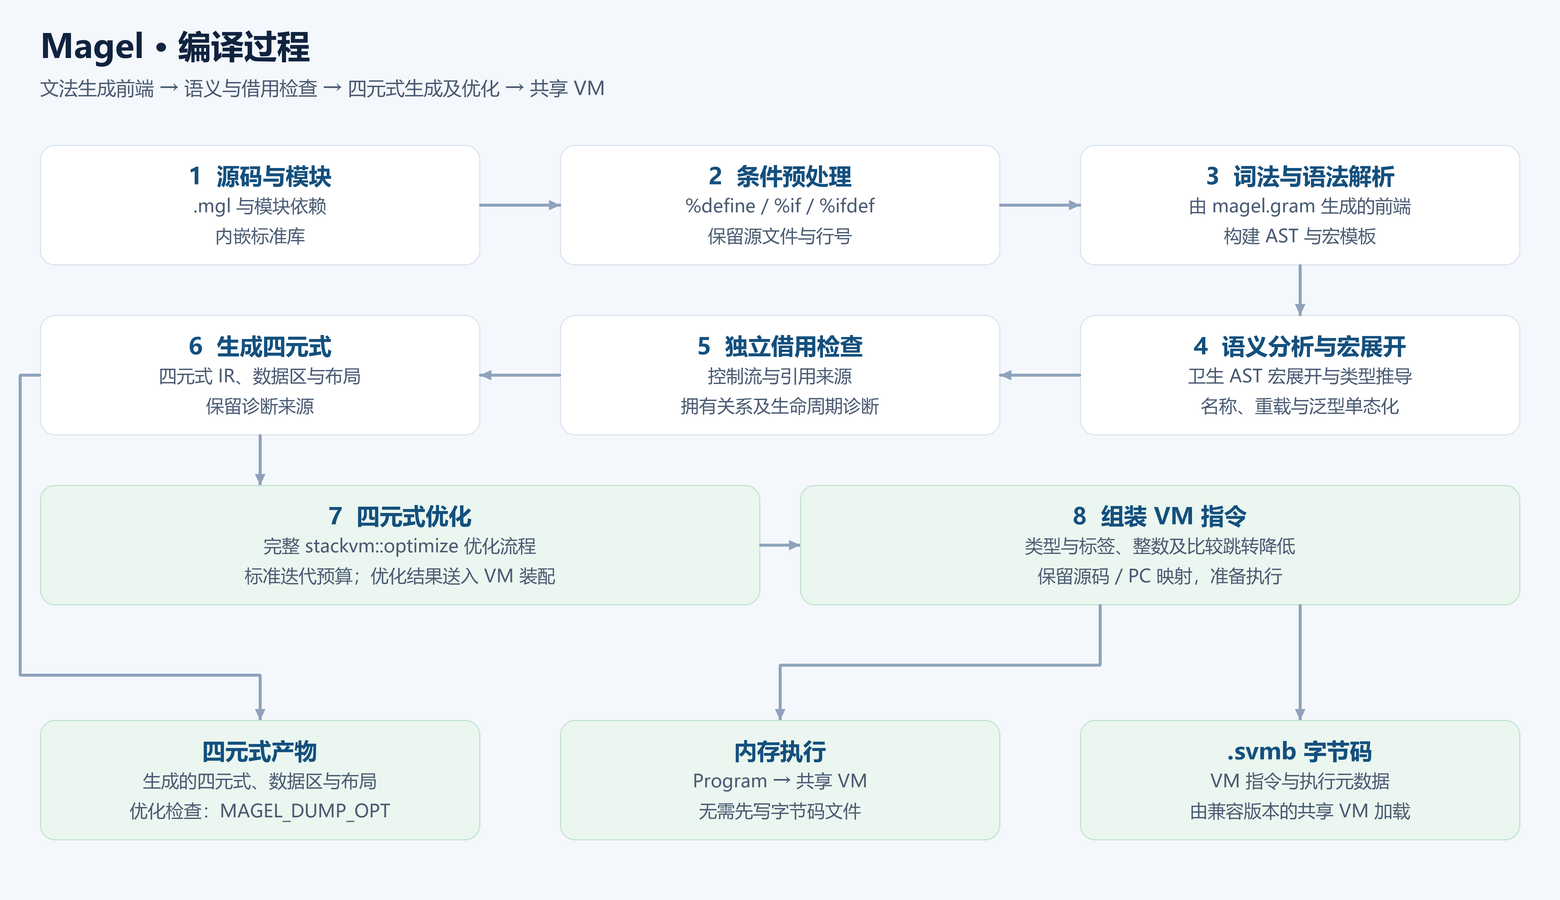
\includegraphics[width=\linewidth]{../images/magel-compilation.png}\par
Magel 编译流程：预处理、解析、语义期宏展开、借用检查、四元式及 VM 装配
\end{center}

四元式是本书所说的 IR。编译器先生成四元式、数据区和布局，供检查或后续装配；执行路径对四元式进行完整优化，再组装 VM 指令。图中的四元式产物出口位于生成阶段，优化结果可通过调试输出检查，二者不要混淆。

再看运行流程。源码运行和字节码运行最终都进入同一套共享 VM。执行准备绑定入口和宿主服务，运行时按指令操作数据、调用原生服务，并处理预算、错误与资源清理。

\begin{center}
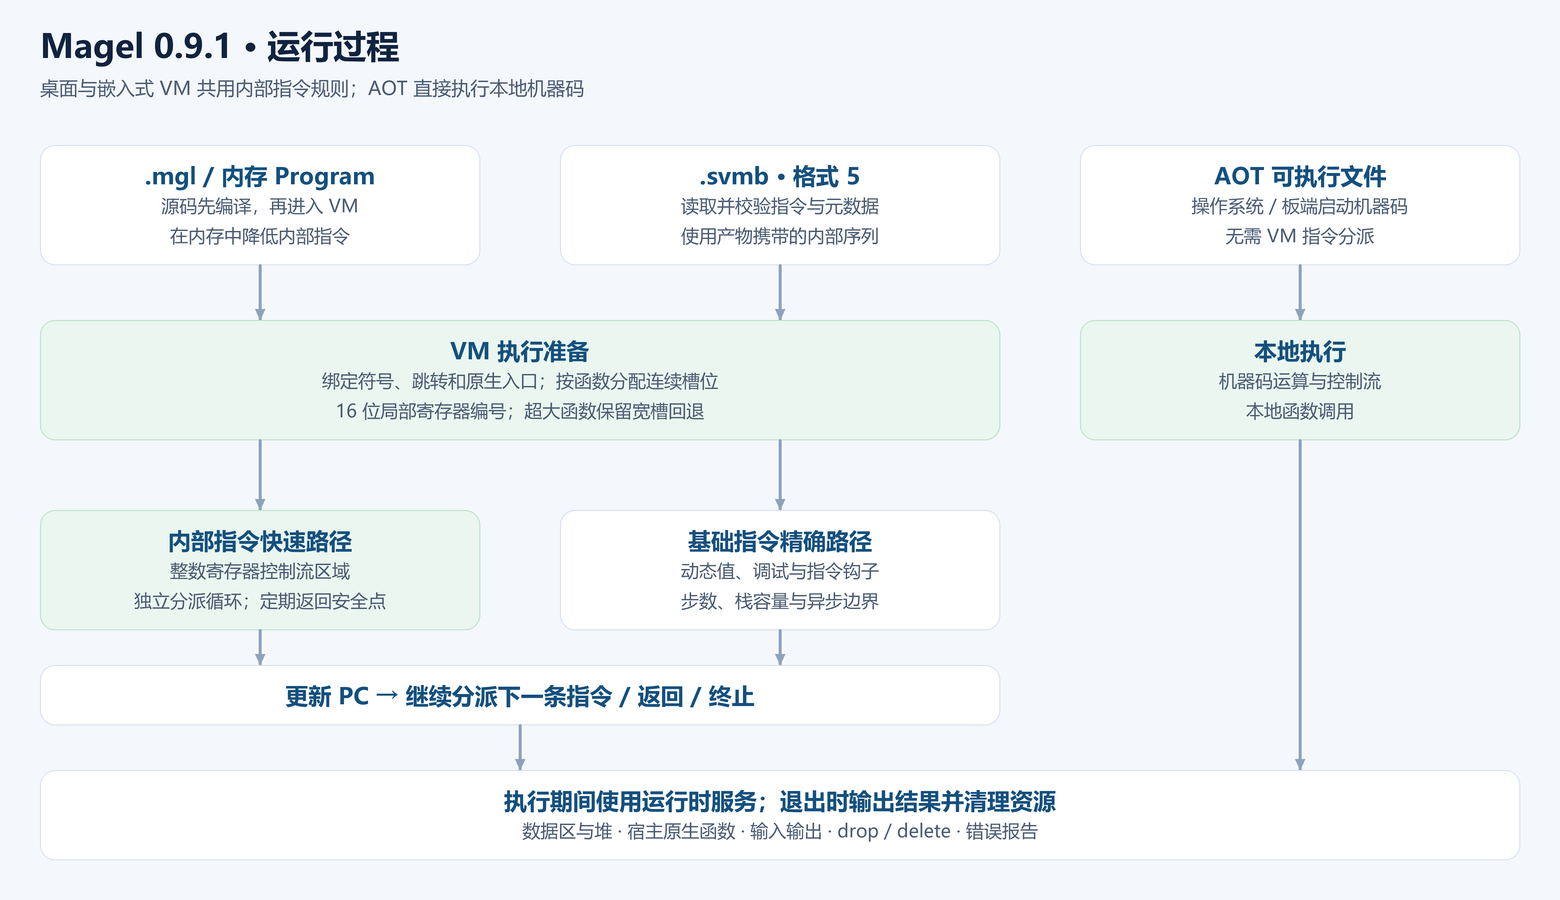
\includegraphics[width=\linewidth]{../images/magel-execution.png}\par
Magel 虚拟机流程：程序加载、执行准备、寄存器快速路径、精确路径与运行时服务
\end{center}

寄存器核心、融合与其他优化属于 VM 内部实现；调试和精确边界按需要使用相应路径。使用者先关注输入、输出和错误，不必在第一章记住所有实现名词。资源与作用域见第 8 章，实际交付边界见第 22 章。

两张图与仓库 README 使用相同绘图脚本生成。内嵌手册导出时携带图片，PDF 也直接收录图片，所以离线阅读不依赖网络。

\section{小结}

这一章你认识了：

\begin{itemize}

\item 入口函数固定叫 \texttt{main}，返回 \texttt{int64} 或 \texttt{void}；\texttt{void main} 正常完成时退出码为 0，panic 仍失败；

\item \texttt{println(\allowbreak{}.\allowbreak{}.\allowbreak{}.\allowbreak{})\allowbreak{}} 打印一行，来自核心库，不用 import；

\item 分号断句、花括号划范围，和 C 系语言一样；

\item \texttt{magel run} 跑，\texttt{magel check} 只查；

\item 报错会给出行列位置和画了波浪线的源码，而且大多在编译期就报出来了。

\end{itemize}

还有一件事本章没讲：\texttt{println} 为什么不用 \texttt{import}？因为它属于核心模块 \texttt{lang}，而 \texttt{lang} 是自动加载的。别的模块就没这个待遇了，第 18 章会讲清楚。

\section{下一步}

光看「Hello, Magel」是学不会编程的。下一章我们写一个真的有用的小程序：键盘猜数字。它会用到变量、输入、循环和分支——四个最基础的积木，而且你会看到它们是怎么串在一起的。

翻到\hyperref[ch:02]{第 2 章 猜数字}。

\section{边界与验证}

通过语法和类型检查，只能证明对应静态检查通过。程序是否产生预期输出、是否访问了外部资源，需要运行验证；外部输入变化也可能使后续运行失败。

\section{习题}

前两题用于理解和基本实现，第三题检查边界，最后一题为综合挑战。先独立完成，再核对参考解答。

\begin{enumerate}

\item 解释检查成功与运行结果正确之间的区别。

\item 把欢迎程序改为输出两行，分别为自己的名字和 Hello, Magel!。

\item 删掉语句末尾的分号，检查诊断位置，再修复。

\item 挑战：写出一个检查成功、运行时断言失败的完整程序。

\end{enumerate}

\subsection*{参考解答与验收要点}

\begin{enumerate}

\item 检查不执行全部业务路径；运行时还可能发生断言、输入或宿主错误。至少分别记录检查状态、退出状态和实际输出。

\item 使用两次 println，逐行对照输出；不要把编辑器显示的文字当成程序输出。

\item 这是语法错误练习，应在检查阶段失败。记录文件、行列和具体缺失内容，不把整条诊断文案写死。

\item 在 main 内调用 assert(false)，检查成功但执行失败；将它作为故意失败用例单独保存。

\end{enumerate}

\section{番外：皇帝的新程序}

改编自安徒生《皇帝的新装》，以下为编程主题的独立改写。

皇帝最爱新程序，早朝先问今日添了几个功能。两个裁缝进宫，说能编出天下最快的程序，只有不称职的大臣看不见运行结果。

老臣奉命验收，看见屏幕空空，心中一惊。他问裁缝为何没有输出。裁缝指着一页没有错误的检查记录：“只有懂编译的人才看得出。”老臣便在验收书上写了“运行极快”。

第二位大臣更谨慎，亲眼看见源码通过检查，才回去报告：“臣已确认，全无错误。”他没有按下运行键，怕显得自己不懂。

游行那天，皇帝抱着空屏幕走过大街。百姓都赞叹程序的速度；一个孩子问：“它究竟做了什么？”人群渐渐安静。皇帝叫人运行，屏幕这才显出第一行字。他想停下游行，可仪仗已经走到了街口，大臣们仍举着写有“验收通过”的牌子。

\subsection*{技术对照}

通过语法和类型检查，只能证明对应静态检查通过。程序是否产生预期输出、是否访问了外部资源，需要运行验证；外部输入变化也可能使后续运行失败。
